% ============================================================================
% LISTA DE ILUSTRAÇÕES
% ============================================================================
%
% Este arquivo contém a definição de todas as ilustrações que devem ser incluídas
% no documento. Para adicionar uma nova ilustração:
%
% 1. Adicione a ilustração na pasta correta /ilustracoes/[figuras,fotografias,graficos,quadros]
% 2. Adicione a devida seção \begin{figura}...\end{figura} ou \begin{quadro}...\end{quadro}
%    em \includegraphics referencie o caminho da figura. Ex: ilustrações/figuras/nome_da_figura.png
%    utilize o comando \legenda{} para a legenda e \fonte{} para a fonte.
%    utilize o comando \label{} para o rótulo da figura ou quadro, a ser referenciada no artigo. Ex: \label{figura:NomeDoRótulo} ou \label{quadro:NomeDoRótulo}
%
% 3. No documento principal, referencie a ilustração utilizando \ref{figura:NomeDoRótulo} ou \ref{quadro:NomeDoRótulo}
%
% Os apêndices serão incluídos na ordem listada abaixo.
% ============================================================================


% FIGURAS ======================================================================
\begin{figura}[h!]
  \centering
  \addfigura
  \includegraphics[width=1\textwidth]{ilustracoes/figuras/Estrutura de trabalho acadêmico.png}
  \legenda{Estrutura de trabalhos acadêmicos, monografias e relatórios de estágio}
  \fonte{O autor}
  \label{figura:EstruturaTrabalhoAcademico}
\end{figura}

\begin{figura}[h!]
  \centering
  \addfigura
  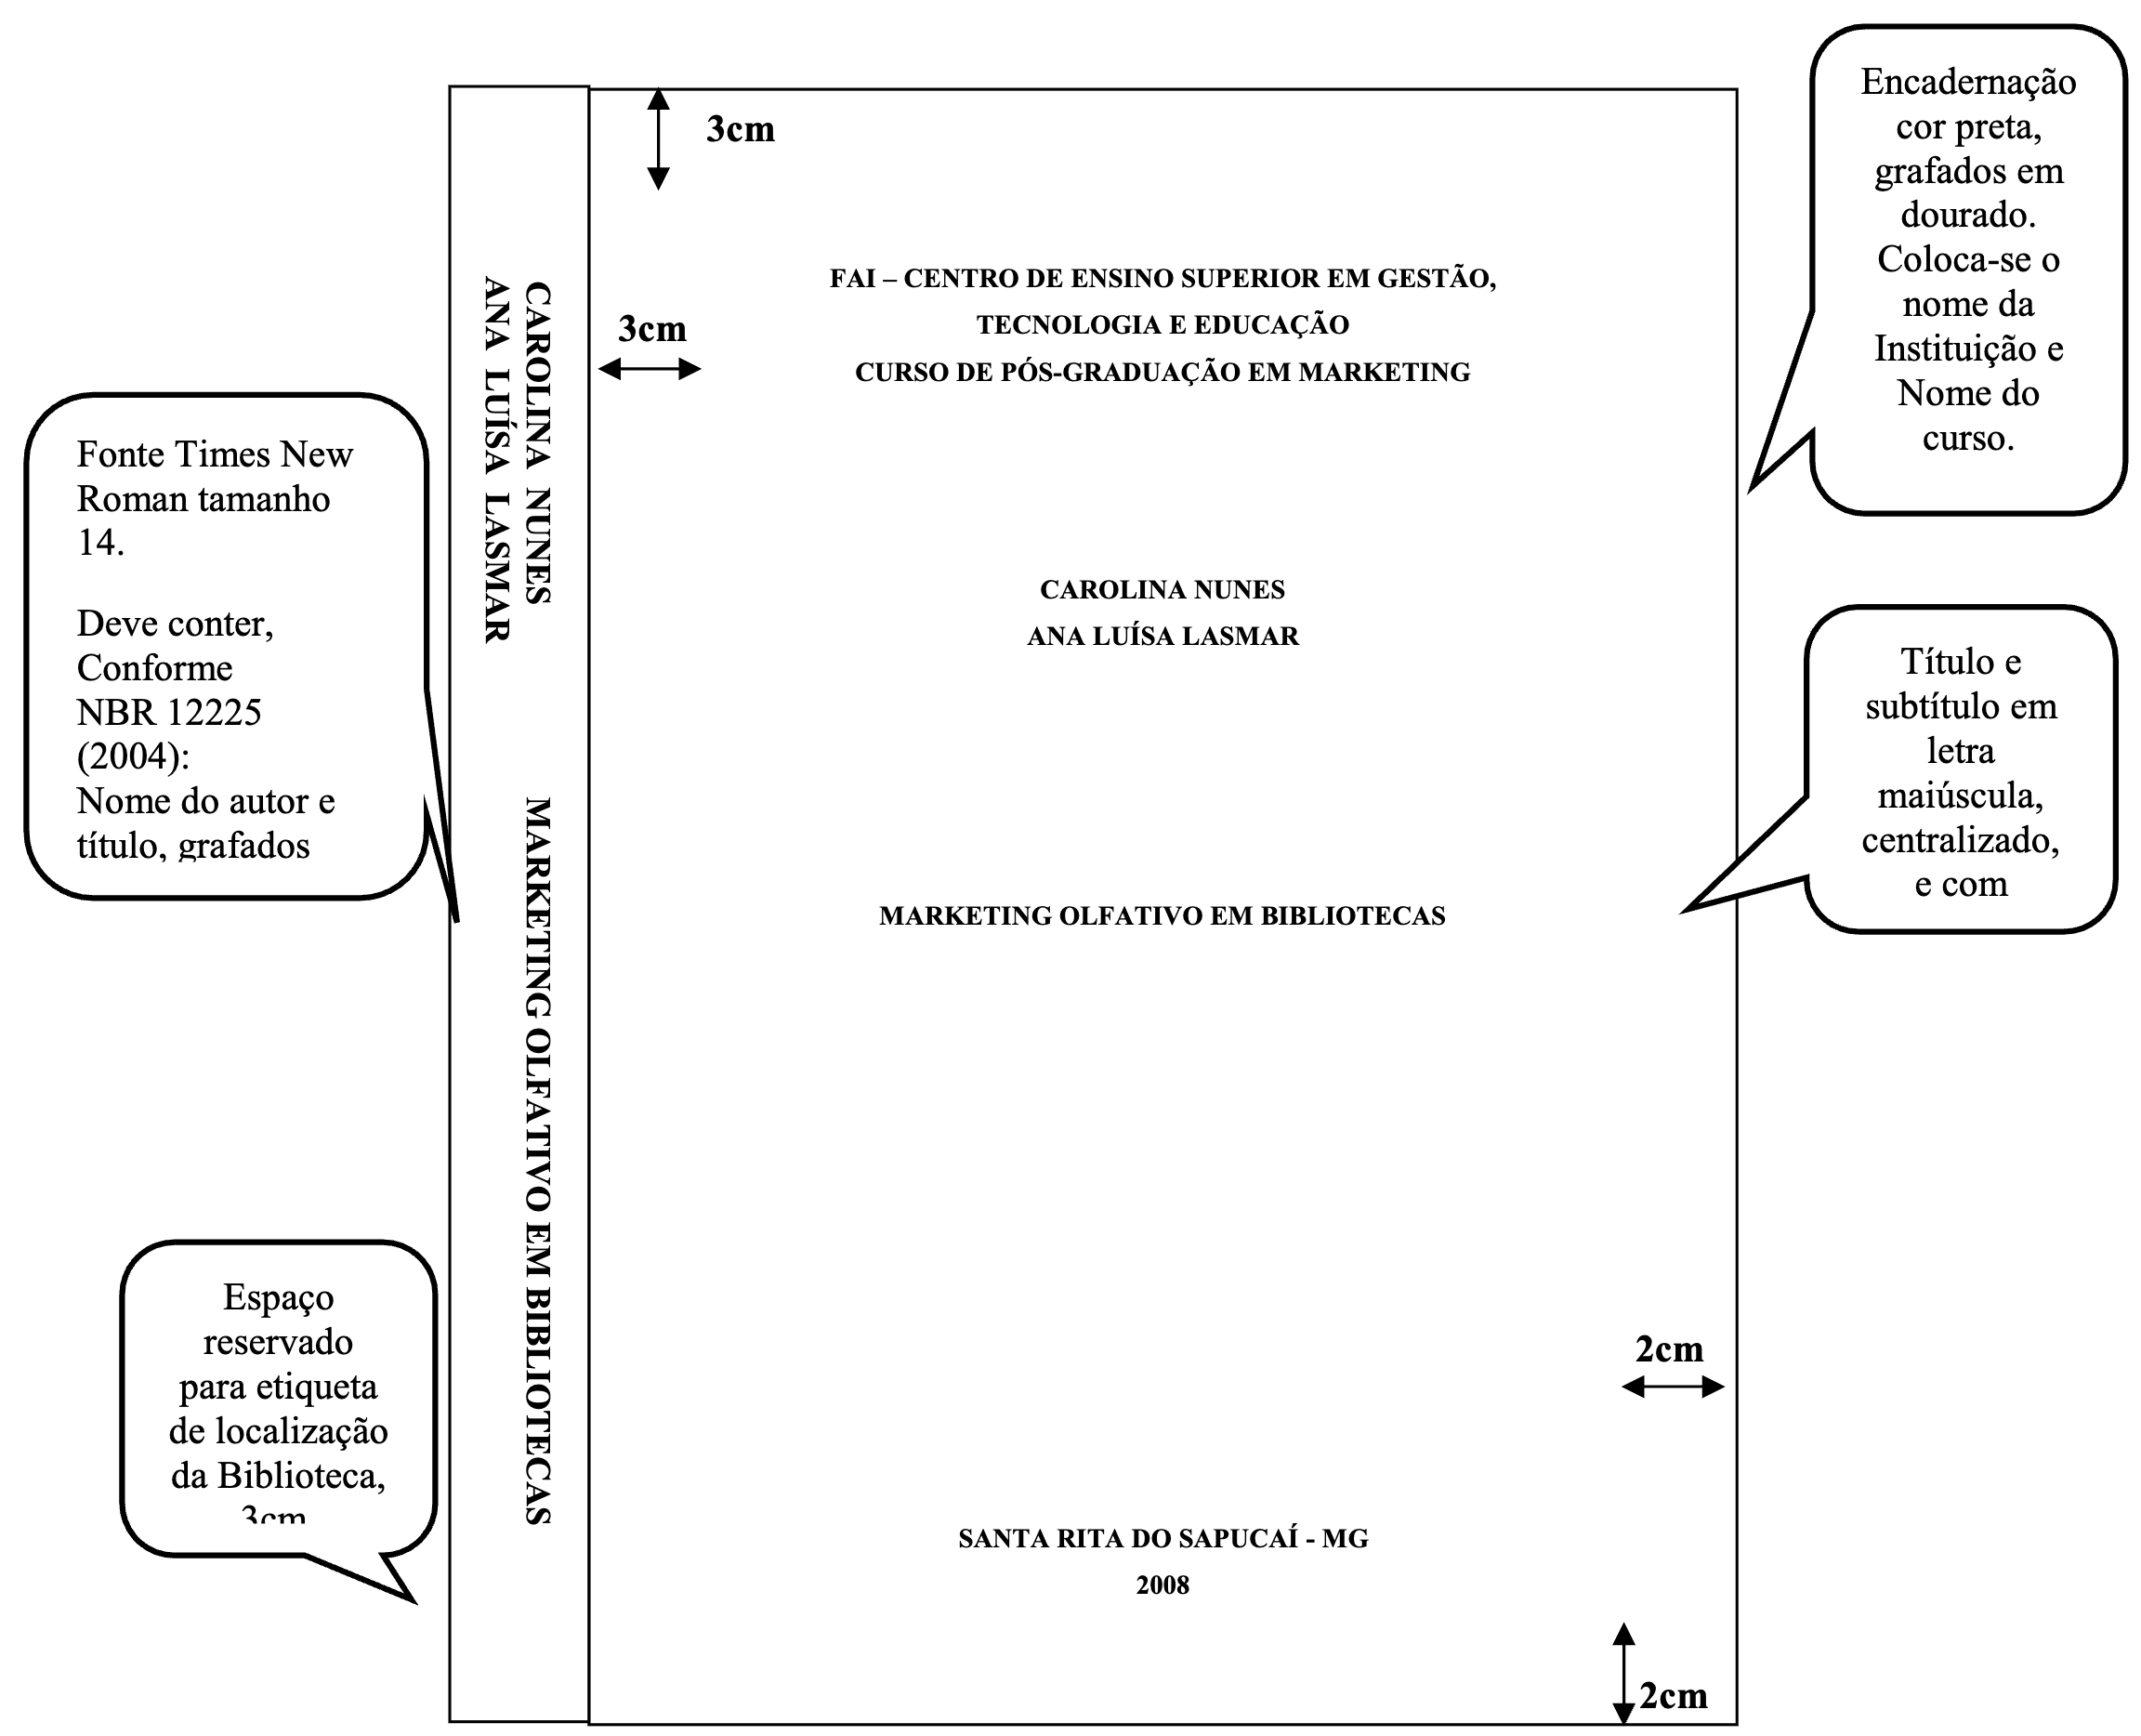
\includegraphics[width=1\textwidth]{ilustracoes/figuras/Modelo de Capa e Lombada.png}
  \legenda{Modelo de Capa e Lombada}
  \fonte{Elaboração própria}
  \label{figura:ModeloDeCapaELombada}
\end{figura}

\begin{figura}[h!]
  \centering
  \addfigura
  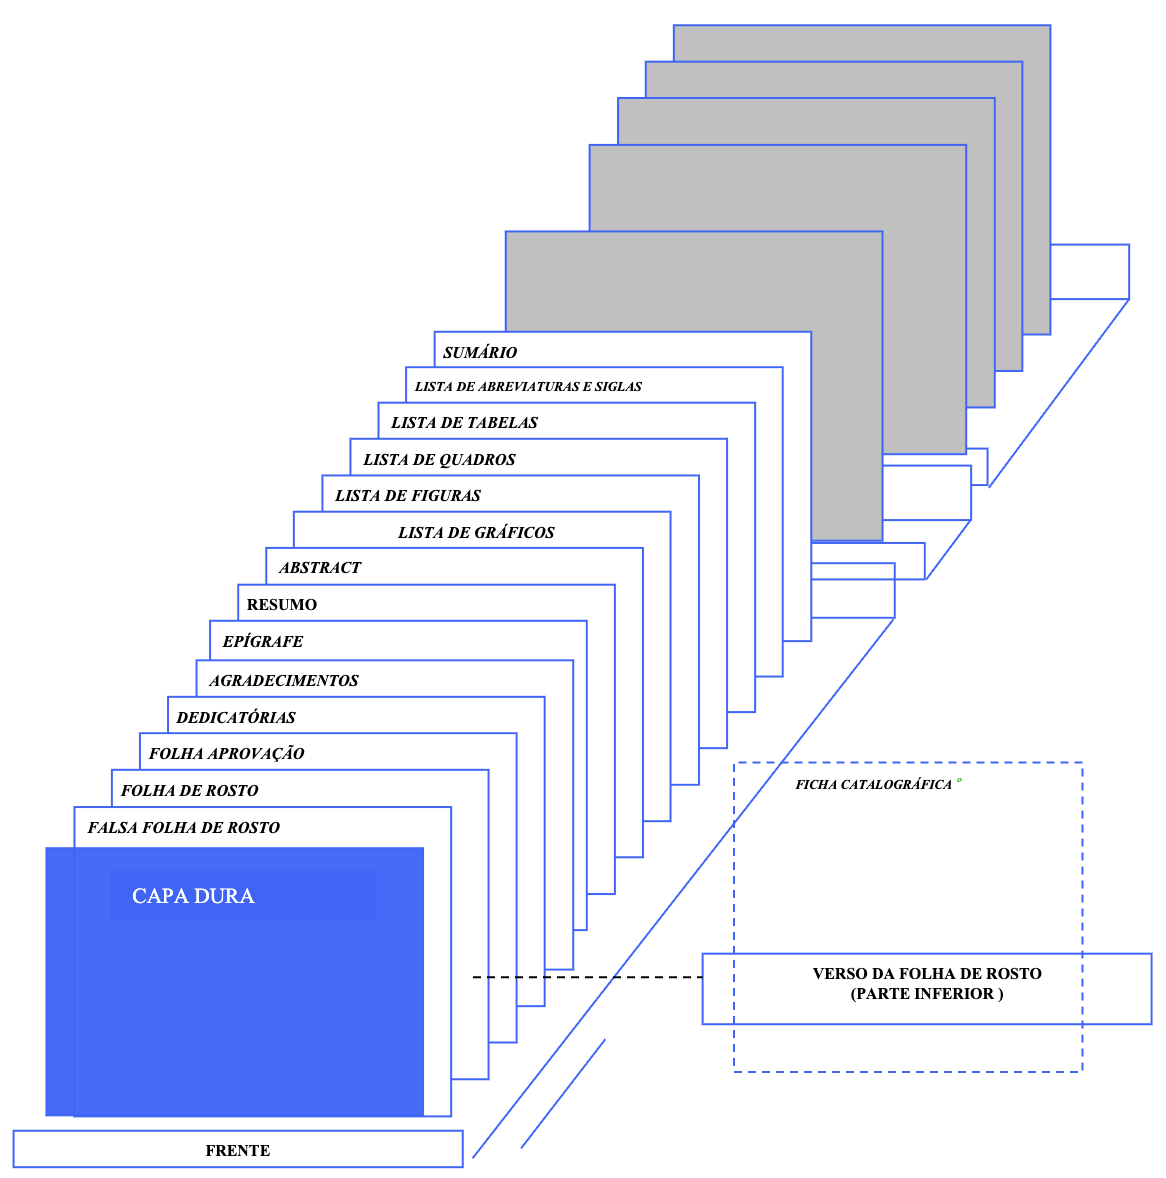
\includegraphics[width=1\textwidth]{ilustracoes/figuras/Elementos Pre Textuais.png}
  \legenda{Elementos Pré-Textuais}
  \fonte{Elaboração própria}
  \label{figura:ElementosPreTextuais}
\end{figura}


% QUADROS ====================================================================
\begin{quadro} [h!]
  \centering
  \addquadro
  \includegraphics[width=1\textwidth]{ilustracoes/quadros/Especificação de Elementos.png}
  \legenda{Especificação de elementos em função do tipo de trabalho}
  \fonte{Equipe do Núcleo de Pós-Graduação da FAI}
  \label{quadro:EspecificacaoElementos}
\end{quadro}


% FOTOGRAFIAS =================================================================


% GRÁFICOS ====================================================================
